The expected yield for processes with FNP leptons, 
estimated with the method described in 
Sections~\ref{sec:bkg.red.mct} and~\ref{subsec:fakes_mctemplate}, 
are presented in Table~\ref{tab:fakes_sr_yields} for the signal regions. 
The estimates are all found to be consistent with each other. 

The final numbers retained for the fake lepton background estimate,
shown in Table~\ref{tab:fakes_sr_yields}
are taken as the weighted-average of the predictions from the matrix method 
and the MC template; 
the weights are based on the statistical component, and the systematic 
uncertainties are propagated 
assuming conservatively a full correlation between the two methods, 
although they are in fact largely independent. 
The central value along with the statistical and systematic uncertainties 
are therefore: 

\begin{equation}
\begin{aligned}
& \left(w\zeta_1 + (1-w)\zeta_2\right) 
\pm \sqrt{w^2\left(\Delta\zeta_1^\text{(stat)}\right)^2 + (1-w)^2\left(\Delta\zeta_2^\text{(stat)}\right)^2} \\
&\hspace{3.225cm} \pm \left(w\Delta\zeta_1^\text{(syst)} + (1-w)\Delta\zeta_2^\text{(syst)}\right)\\
&\qquad\text{ with }w=\frac{\left(\Delta\zeta_2^\text{(stat)}\right)^2}{\left(\Delta\zeta_1^\text{(stat)}\right)^2+\left(\Delta\zeta_2^\text{(stat)}\right)^2}\notag
\end{aligned}
\end{equation}

When the estimated value is too small (below 0.15), the expected yield is set
 to $0.15\pm 0.15$, 
to cover for possibilities of an under-fluctuation of the number of
 baseline-not-signal leptons 
when applying the matrix method, as well as lack of statistics in the MC 
samples for the other method. 

\begin{table}[!htb]
  \caption{Expected yields for background processes with FNP leptons
    shown for 36 \ifb. Uncertainties include all statistical and systematic 
sources for the nominal estimate . 
}
\label{tab:fakes_sr_yields}
\centering
\resizebox{\textwidth}{!}{
\begin{tabular}{|c||c|c||c|}\hline
      Region &              Matrix method   &   Template method   &     Retained estimate  \\\hline
    Rpc2L0bH & $ 0.83 \pm  0.56 \pm  0.74$  &  $1.00 \pm 0.96 \pm 0.81$ &  $ 0.87 \pm  0.48 \pm  0.76$  \\
    Rpc2L0bS & $ 1.51 \pm  0.60 \pm  0.66$  &  $1.68 \pm 1.02 \pm 1.26$  &  $ 1.55 \pm  0.52 \pm  0.81$  \\
    Rpc2L1bH & $ 3.54 \pm  1.62 \pm  3.12$  &  $2.07 \pm 0.63 \pm 1.56$  &  $ 2.26 \pm  0.59 \pm  1.76$  \\
    Rpc2L1bS & $ 2.65 \pm  1.21 \pm  1.89$  &  $02.33 \pm 01.17 \pm 02.10$  & $ 2.48 \pm  0.84 \pm  2.00$  \\ 
    Rpc2L2bH & $-0.11 \pm  0.11 \pm  0.18$  &  $<0.5$  &  $ 0.15 \pm  0.15 \pm  0.00$  \\
    Rpc2L2bS & $ 1.31 \pm  1.07 \pm  1.65$  &  $0.41 \pm 0.33 \pm 0.45$ &  $ 0.49 \pm  0.32 \pm  0.55$  \\
    Rpc2Lsoft1b & $ 4.75 \pm  1.42 \pm  2.64$  &  $2.48 \pm 1.32 \pm 1.86$  &  $ 3.53 \pm  0.97 \pm  2.22$  \\
    Rpc2Lsoft2b & $ 1.91 \pm  1.18 \pm  1.63$  &  $1.66 \pm 0.66 \pm 1.28$ &  $ 1.72 \pm  0.58 \pm  1.36$  \\
    Rpc3L0bH & $-0.01 \pm  0.11 \pm  0.10$  &  $<0.5$                     &  $ 0.15 \pm  0.15 \pm  0.00$  \\
    Rpc3L0bS & $ 2.31 \pm  1.50 \pm  2.63$  &  $0.21 \pm 0.15 \pm 0.16$   &  $ 0.23 \pm  0.15 \pm  0.18$  \\
    Rpc3L1bH & $ 0.57 \pm  0.43 \pm  0.50$  &  $0.42 \pm 0.29 \pm 0.32$  
                      &  $ 0.47 \pm  0.24 \pm  0.38$  \\
    Rpc3L1bS & $ 4.94 \pm  1.83 \pm  2.96$  &  $3.55 \pm 1.80 \pm 2.76$   &  $ 4.23 \pm  1.28 \pm  2.86$  \\
    Rpc3LSS1b & $-0.18 \pm  1.24 \pm  2.85$  &  $0.90 \pm 0.14 \pm 0.69$  
    &  $ 0.89 \pm  0.14 \pm  0.72$  \\
\hline
\hline
\end{tabular}
}
\end{table}


\begin{figure}[htb!]
\centering
\begin{subfigure}[t]{0.66\textwidth}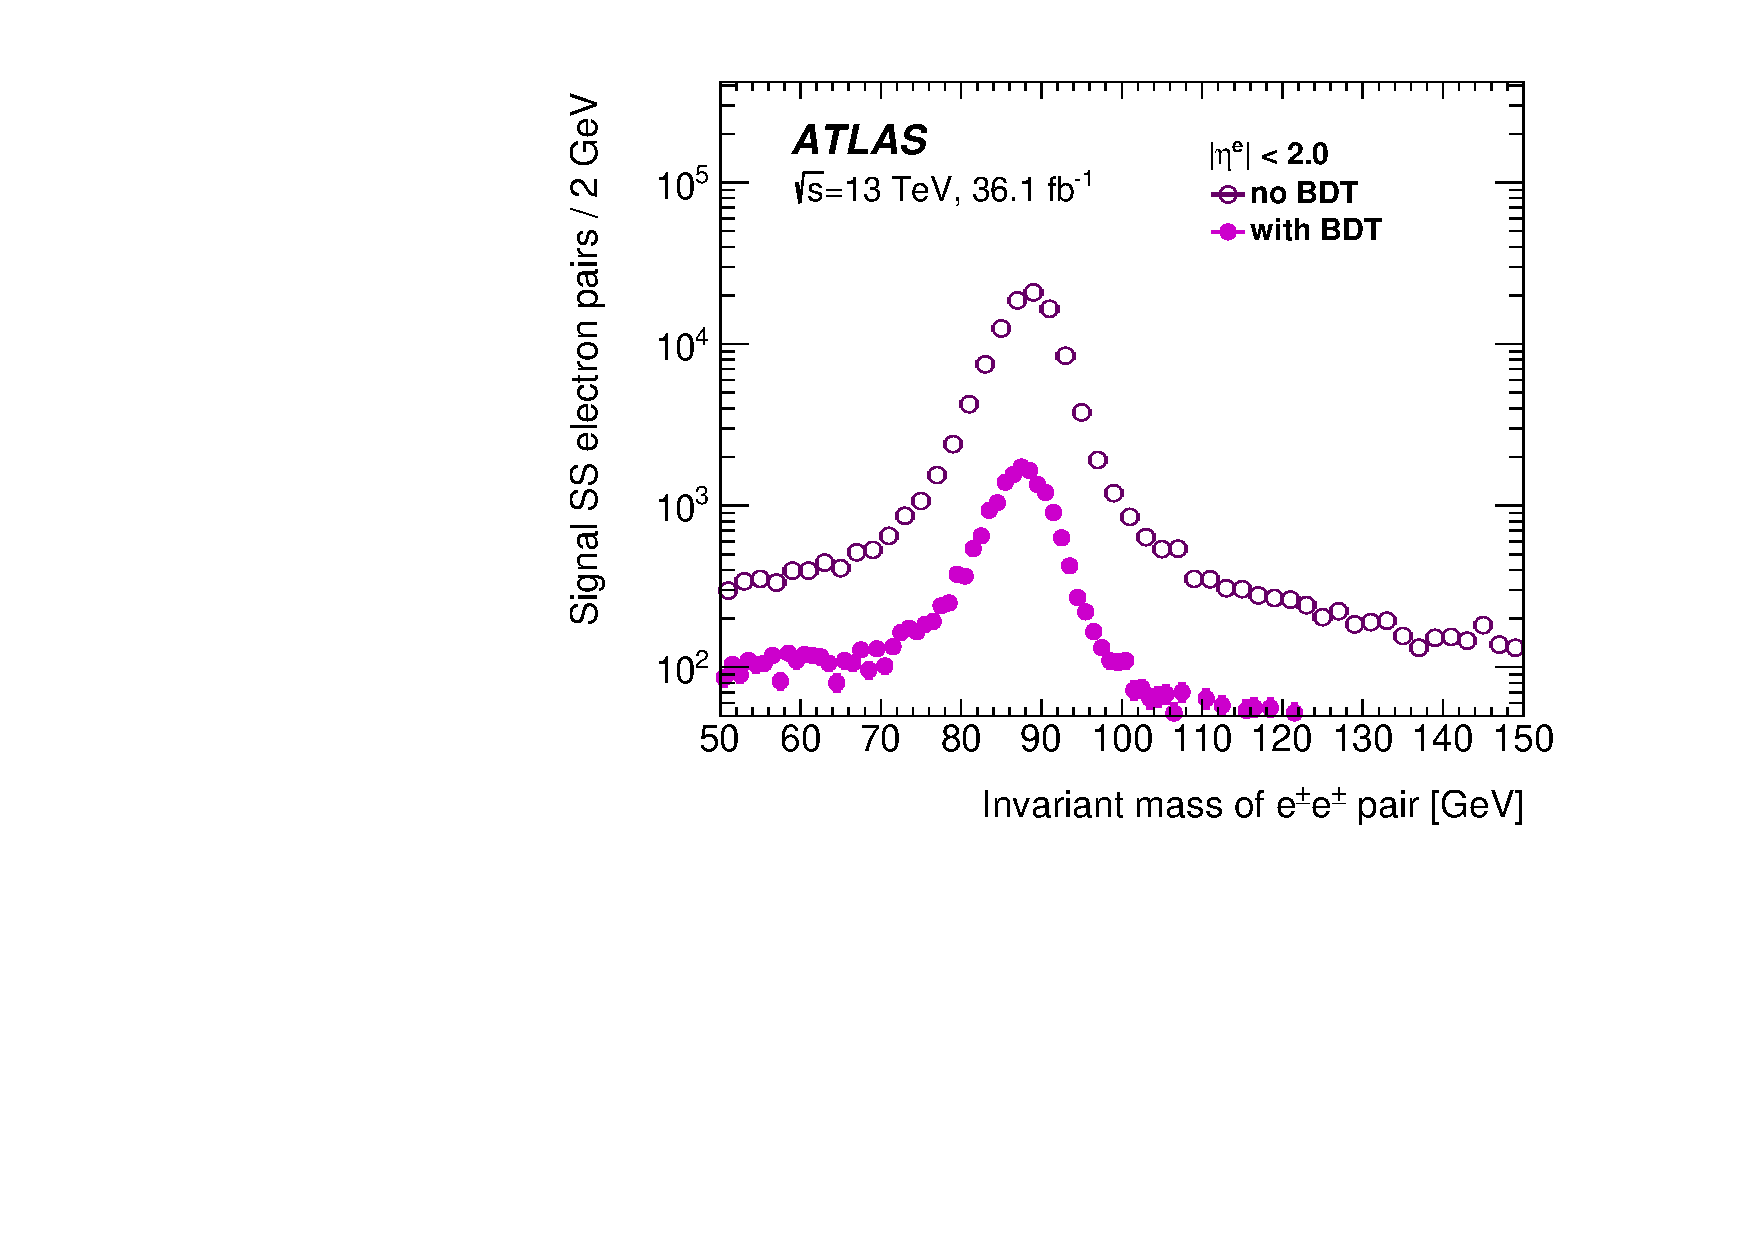
\includegraphics[width=\textwidth]{ETA_SS_BDTEL}\end{subfigure}
\caption{Invariant mass of the signal $e^{\pm} e^{\pm}$ pair distribution with (full markers) and without (open markers) charge-flip electron BDT selection applied.
}
\label{fig:ETA_SS_BDTEL}
\end{figure}



\begin{table}[!htb]
\caption{Expected yields for background processes with charge-flipped electrons
in the signal regions. Comparison between the data-driven and the MC template
estimates.
Uncertainties include all statistical and systematic sources. 
Charge-flip processes do not contribute to signal regions which require $\ge 3$ leptons. 
}
\label{tab:chargeflip_sr_yields}
\centering
\begin{tabular}{|c||c|c|}\hline
 Region      &   Weighted OS data          &     Template method \\\hline
    Rpc2L0bH & $ 0.01 \pm  0.00 \pm  0.00$ & $<0.4$ \\
    Rpc2L0bS & $ 0.05 \pm  0.01 \pm  0.01$ & $ 00.02 \pm 00.02 \pm 00.00 $ \\
    Rpc2L1bH & $ 0.25 \pm  0.03 \pm  0.04$ & $ 00.21 \pm 00.32 \pm 00.16 $ \\
    Rpc2L1bS & $ 0.25 \pm  0.02 \pm  0.04$ & $ 00.35 \pm 00.37 \pm 00.26 $ \\
    Rpc2L2bH & $ 0.02 \pm  0.01 \pm  0.00$ & $<0.4$ \\
    Rpc2L2bS & $ 0.10 \pm  0.01 \pm  0.02$ & $<0.4$ \\
 Rpc2Lsoft1b & $ 0.08 \pm  0.01 \pm  0.02$ & $<0.4$ \\
 Rpc2Lsoft2b & $ 0.08 \pm  0.01 \pm  0.02$ & $<0.4$ \\
   Rpc3LSS1b & $ 0.39 \pm  0.03 \pm  0.07$ & $ 00.81 \pm 00.53 \pm 00.34 $ \\
\hline
\hline
\end{tabular}
\end{table}
